% LaTeX template for a short report (written for MSES scenario modelling)
% uses LaTeX documentclass "article" for use of sections (not chapter) and References (not Bibliography)
% for Chapters and Bibliography use "documentclass "report
\documentclass[10pt]{article}   % Use article class with 10pt letter
%\documentclass[10pt]{report}
\usepackage[utf8]{inputenc}

%\usepackage[T1]{fontenc}  % 8-bit encoding, helps hyphenation of accented characters -
% https://tex.stackexchange.com/a/677/42066

% Use A4 paper and set margins:
%\usepackage[a4paper, twoside, top=2.0cm, left=3.0cm, bottom=2.0cm, right=2.0cm]{geometry}
\usepackage[a4paper, twoside, top=2.0cm, left=2.0cm, bottom=2.0cm, right=2.0cm]{geometry}
%\usepackage[a4paper, top=2.5cm, left=2.5cm, bottom=2.5cm, right=2.5cm]{geometry}

\usepackage[english]{babel}  % Hyphenation and more for English

\usepackage{pgf}      % Include graphics inside figures using \pgfimage
\usepackage[font=small, labelfont=bf]{caption}  % Stylize figure, table, etc. captions

\usepackage{parskip}         % Replace paragraph indentations with white lines
\usepackage[hyphens]{url}    % Take care of urls, e.g. wrapping in the Bibliography (hyphens: also break at -)

\usepackage{xspace}   % \xspace saves the user from having to type \  or {} after a macro name in text.

% Use the appendix package for nicer appendices:
%\usepackage[toc,page]{appendix}  % MvdS
\usepackage[titletoc]{appendix}
%\usepackage[toc,page,title]{appendix}  % Use \begin{appendices} ... \end{} iso \appendix

% \usepackage[numbib,numindex]{tocbibind}  % Add ToC, List of Figures/Tables/Code listings, Bibliography and Index to ToC
% \usepackage[]{tocbibind}       % Add ToC, List of Figures/Tables/Code listings, Bibliography and Index to ToC
\usepackage[nottoc]{tocbibind}   % ToC without extra "Contents" entry...

\usepackage{amsmath,amssymb,bbm}
\usepackage{enumerate}         % Choose alternative numberings, e.g. \begin{enumerate}[a.]

\usepackage{listings}          % Code listings
\usepackage[section, above, below]{placeins}  % \FloatBarrier - flush floats before \section by default
% \usepackage{pgf}               % Figures

\usepackage{color}
\definecolor{lightgrey}{rgb}{0.9,0.9,0.9}
\definecolor{darkgreen}{rgb}{0.0,0.6,0.0}

% Citations:

% option1: use natbib/bibtex with MvdS_number_url.bst
%\usepackage[numbers, square]{natbib}  % Use numbered citations with square brackets
%\bibliographystyle{MvdS_number_url}  % Use [1], print url = field  (plain doesn't print urls)

%option2: use biblatex/biber without *.bst file
\usepackage[backend=biber, style=numeric, citestyle=numeric-comp, sorting=none]{biblatex} 
\setlength\bibitemsep{0.5\baselineskip}
\usepackage{csquotes}

% \bibliography{mybibliography} % old-style for backward comp. in preamble for biblatex/bibtex
\addbibresource{mybibliography.bib}  % new syntax for BibLaTeX


\usepackage{fancybox}  % Use \ovalbox for key strokes

\newcommand{\ldf}{\usefont{OT1}{cmr}{m}{n}}     % Select default LaTeX font - Computer Modern Roman
%\newcommand{\ldf}{\usefont{OT1}{cmss}{m}{n}}     % Select default LaTeX font - Computer Modern Sans
%\newcommand{\ldf}{\usefont{OT1}{phv}{m}{n}}     % Select default LaTeX font - Helvetica
\newcommand{\ttbf}{\usefont{OT1}{lmtt}{bx}{n}}  % Select bold typewriter font

%\usepackage[font=sf]{caption}  % Use sans-serif font for float captions - not exactly Helvetica



\newcommand{\note}[1]{\color{red}\textbf{#1}\color{black}\xspace}
\newcommand{\marc}[1]{\color{red}\textbf{Marc: #1}\color{black}\xspace}

\newcommand{\myChapter}[1]{
  \chapter{#1}
  \minitoc  % Create a ToC of this chapter
}


% General expressions:
\newcommand{\eg}{\emph{e.g.}\xspace}
\newcommand{\ie}{\emph{i.e.}\xspace}
\newcommand{\etc}{\emph{et cetera}\xspace}
\newcommand{\ff}{\emph{ff}\xspace}

% CLI symbols:
\newcommand{\pipe}{$|$}      % Needed to avoid | in \index{}
\newcommand{\logor}{$|\,|$}  % Needed to avoid | in \index{}
\newcommand{\home}{\url{~}}  % Home directory


% Often used code names:
\newcommand{\NULL}{\code{NULL}}
\newcommand{\void}{\code{void}}
\newcommand{\stdout}{\code{stdout}}
\newcommand{\stderr}{\code{stderr}}

% Man pages:
\newcommand{\man}[2]{\texttt{man #1 #2}\xspace}
\newcommand{\mancmd}[1]{\texttt{man #1}\xspace}

% Code:
\newcommand{\prototype}[3]{\hspace*{2em}\texttt{#1} {\ttbf #2\ldf}(\texttt{#3});\xspace}  % function prototype
\newcommand{\var}[2]{\hspace*{2em}\texttt{#1} {\ttbf #2\ldf};\xspace}  % variable declaration
\newcommand{\code}[1]{\texttt{#1}\xspace}  % inline code
\newcommand{\codeb}[1]{\ttbf #1\ldf\xspace}  % inline bold code
\newcommand{\codeline}[1]{\hspace*{2em}\texttt{#1}}  % separate code line

\newcommand{\cli}[1]{\noindent\hspace*{2em}\code{\$ #1}}  % command line input
\newcommand{\clir}[1]{\noindent\hspace*{2em}\code{\# #1}}  % command line input root
\newcommand{\clo}[1]{\noindent\hspace*{2em}\code{#1}}  % command line output
\newcommand{\clitem}[1]{\item[\code{\$}] \code{#1}}  % cli in itemized list, with $ as bullet
\newcommand{\clitemb}[1]{\item[\codeb{\$}] \codeb{#1}}  % cli in itemized list, with $ as bullet - bold

\newcommand{\key}[1]{\Ovalbox{\texttt{#1}}\xspace}  % key press/combination
\newcommand{\keyb}[1]{\Ovalbox{\ttbf #1\ldf}\xspace}  % key press/combination bold


% Heat pumps
\newcommand{\COP}{\mathrm{COP}}  % COP in "math mode"
\newcommand{\COPh}{\COP_{\mathrm{heating}}}  % COP_heating in "math mode"

\newcommand{\Qh}{Q_{\mathrm{H}}}
\newcommand{\Qc}{Q_{\mathrm{C}}}
\newcommand{\Th}{T_{\mathrm{H}}}
\newcommand{\Tc}{T_{\mathrm{C}}}

\newcommand{\Tin}{T_{\mathrm{in}}}
\newcommand{\Tout}{T_{\mathrm{out}}}

\newcommand{\Ph}{P_{\mathrm{heat}}}
\newcommand{\Pheat}{P_{\mathrm{heat}}}
\newcommand{\Pc}{P_{\mathrm{cool}}}
\newcommand{\Pcool}{P_{\mathrm{cool}}}
\newcommand{\Pel}{P_{\mathrm{el}}}

\newcommand{\degr}{^\circ}
\newcommand{\tdeg}{$\degr$\xspace}
\newcommand{\degC}{\degr\mathrm{C}}
\newcommand{\tdegC}{$\degC$\xspace}

  % Custom commands

\usepackage[pdftex]{hyperref}
\hypersetup{
  colorlinks = true,  % They get a red box around them if false, better set colour to black?
  linkcolor = blue,
  filecolor = magenta,
  citecolor = blue,
  urlcolor = blue,
  % linkcolor = black,
  % citecolor = black,
  % urlcolor = black,
  pdftitle = House Model References,
  pdfauthor = Trung Nguyen,
  pdfsubject = House Models,
  pdfkeywords = house - models - Python,
  pdfcreator = TeXStudio pdfLaTeX2 on Windows,
  pdfproducer = TeXStudio pdfLaTeX2 on Windows,
  bookmarksnumbered = true,  % Number sections in PDF toc
}

\usepackage[onehalfspacing]{setspace}
\usepackage{float}

\usepackage{graphicx}
\usepackage{multirow}

%\renewcommand{\thesection}{\arabic{section}}  % needed for documentclass "report" with sections





%Document title, author and date (empty)
\title{Defining the RC network}
\author{Marijn Jongerden\\
HAN University of Applied Sciences\\
Arnhem, The Netherlands}
% \date{}

\begin{document}
	
\ldf  % Set LaTeX default font

% Set up code listing style:
\lstset{
	language=Python,
	% Fonts:
	basicstyle=\ttfamily\footnotesize,
	%keywordstyle=\ttfamily,
	%identifierstyle=,
	%commentstyle=\ttfamily\scriptsize,
	% B/W code:
	% commentstyle=\ttfamily\itshape,  % Italic
	% stringstyle=\ttfamily,
	% identifierstyle=\ttbf,           % Bold typewriter type
	% keywordstyle=\ttbf,              % Bold tt
	% Colour:
	commentstyle=\scriptsize\ttfamily\color{brown},
	stringstyle=\ttfamily\color{darkgreen},
	identifierstyle=\color{blue},
	keywordstyle=\ttfamily\color{red},
	% Spaces:
	showstringspaces=false,
	breaklines=true,
	breakatwhitespace=true,
	% Line numbering:
	numbers=left,
	numberstyle=\tiny,
	stepnumber=2, 
	numbersep=5pt,
	% Frames:
	frame=single,
	frameround=tttt,
	backgroundcolor=\color{lightgrey},
	morekeywords={pthread_create},
}
%\renewcommand{\thelstlisting}{\thechapter.\arabic{lstlisting}}  % This is the default?
%\numberwithin{lstlisting}{section}  % AMSmath: number code listings per section
%\numberwithin{lstlisting}{chapter}  % AMSmath: number code listings per chapter

\ldf

\maketitle
\section{heat network equations}

The following is based on the section 5.10 in the document \texttt{House\_model\_references.pdf}.

\subsection{2R2C revisited: 2R3C}
\label{sec:2R3C}
The 2R2C model as represented in Figure 10 [the 2R-2C representation give in chapter 3 of House\_model\_references] treats the node of the outside temperature ($T_{amb}$) differently from the other nodes, $T_{air}$ and $T_{walls}$.  This representation is inconsistent, and actually incomplete. Implicitly, the model links a source/sink to the node that controls the outdoor temperature. In literature, one can find models in which this source has been made explicit, such as in \cite{achterbos}. It seems that this representation has been lost over time. 

In order to complete the analogy with the other nodes in the model we can connect an additional capacitor ($C_{amb}$). The capacity will be tending to infinity, as we assume the outside temperature does not change due to heat exchange with the house. This idea has been sketched in Figure \ref{fig:2R3C}. In the figure, a temperature source (TS) has been attached to the ambient node, which makes that the temperature will remain at a predefined level.  

\begin{figure}
	\centering
	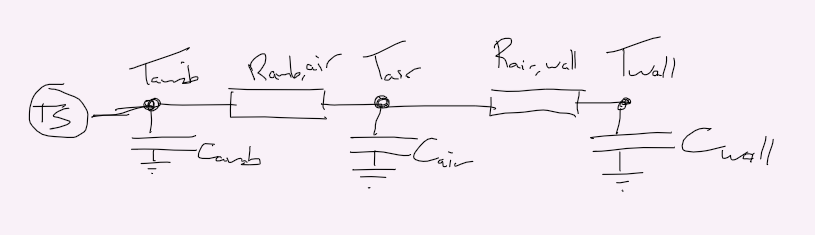
\includegraphics[width=0.7\columnwidth]{Pictures/drawing_2R3C.png}
	\caption[Short title]{2R-3C house model}
	\label{fig:2R3C}
\end{figure} 


Adding the capacitor and the source also will change the equations. Actually, it results in a more structured set of equations. The equations will be as follows:
\begin{equation}
	\mathbf{C} \cdot \boldsymbol{\dot{\theta}} =
	\begin{bmatrix}
		C_{amb} & 0 & 0\\
		0 &  C_{air} & 0   \\
		0 & 0 & C_{wall} 
	\end{bmatrix}
	\cdot
	\begin{bmatrix}
		\frac{dT_{amb}}{dt} \\
		\frac{dT_{air}}{dt} \\
		\frac{dT_{wall}}{dt} 
	\end{bmatrix}
\end{equation}

\begin{equation}
	\mathbf{K} \cdot \boldsymbol{\theta} =
	\begin{bmatrix}
		\frac{1}{R_{amb, air}}  & \frac{-1}{R_{amb,air}} & 0  \\
		\frac{-1}{R_{amb, air}} &  \frac{1}{R_{amb, air}} + \frac{1}{R_{air,wall}} &  \frac{-1}{R_{air,wall}} \\
		 0 & \frac{-1}{R_{air, wall}}  & \frac{1}{R_{air,wall}} 
	\end{bmatrix}
	\cdot
	\begin{bmatrix}
		T_{amb} \\
		T_{air} \\
		T_{wall}
	\end{bmatrix}
\end{equation}

\begin{equation}
	\mathbf{\dot{q}} =
	\begin{bmatrix}
		\dot{Q}_{amb}\\
		\dot{Q}_{air} \\
		\dot{Q}_{wall} 
	\end{bmatrix}
\end{equation}

In the equations we now see that the matrix $K$ represents the interaction between the different heat capacities.  The off-diagonal elements are equal to (minus) conductance factor $\frac{-1}{R}$ between the respective connected nodes. The structure of $K$ is such that the sum over the rows will always be zero, where the diagonal elements equal the negative sum of the off-diagonal elements.

The vector $\dot{q}$ contains all heat sources (and sinks). 

Generalizing the idea above, alternative models can be easily constructed using an underlying graph. In the graph each node is labeled with a heat capacity $C_i$, and temperature $T_i$. Nodes $i$ and $j$ can be connected by an edge labeled with $R_{i,j}$, where $\frac{1}{R_{i,j}}$ represents the heat conductance between the two nodes. The $K$-matrix is the connectivity matrix of the graph, where $K_{i,j} = \frac{-1}{R_{i,j}}$. The diagonal elements, $K_{i,i}$ are set such that the sums over the rows will be equal to zero.
 

Additionally, each node can be connected to a source (or sink). Two types of sources are available. A "temperature source" represents a source that will keep the temperature of the connected node constant within the considered time interval. This source type can be used to set the ambient temperature based on a temperature profile like provided in the NEN5060. It is possible to have multiple temperature sources, but per node only one temperature source can be connected. Another example for a potential temperature source might be the ground temperature, when the heat loss through the floor is to be included explicitly in the model.    

A heat source represents a source that will provide a continuous constant energy flow into the node within the considered time interval. This source type can be used to represent the inflow of energy by for example the sun. 

\section{process for defining the network for modeling}
In order to define a new heat network the following steps need to be followed.
\begin{itemize}
\item Make a drawing of the network, with all its desired heat capacitors and  heat conductors.
\item Identify the nodes that have a predefined temperature, and connect a temperature source in the drawing.
\item Label the $n$ capacitors with a number running from 0 to $n-1$, starting with the capacitors with a predefined temperature. 
\item In the excel file which is used to create the input file the capacities need to be listed with a name and a value in [J/K], as shown in Figure \ref{fig:snip_excel}. For the capacitors connected to a temperature source the capacity needs to be set to "inf", as this ensures that the temperature remains constant. 
\item For the capacitors connected to a temperature source, the prescribed temperature profile needs to be provided. Since this temperature profile, and especially the timestamps in the profile,  needs to be compatible to the other profiles that will be used within the model (for example the NEN weather data), I propose to have all these profiles defined in \emph{one} input-file. A column labeled with the capacity-name will give a clear link between the capacity and its prescribed temperatures. \emph{Note that}, the time granularity will be limited to 1 hour due to the limitations of the NEN, which will be used for the ambient temperature. 

(An option could be to include these profiles in a separate tab in the input excel file, possibly including the other columns used from the NEN, and use this as resource.) 
\item The conductances are defined by a triplet of numbers. The first two numbers are the labels of the connected capacitors, the third gives the heat conductance value in [W/K], as shown in Figure \ref{fig:snip_excel}.  
\end{itemize}


\begin{figure}
	\centering
	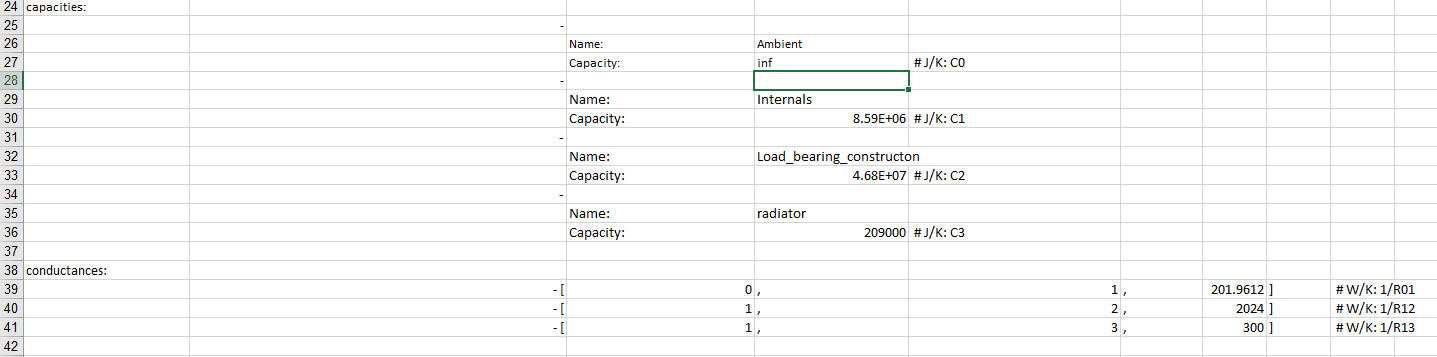
\includegraphics[width=0.95\columnwidth]{Pictures/snip_excel}
	\caption[Short title]{defining capacities and conductances in the excel input file}
	\label{fig:snip_excel}
\end{figure} 


From the resulting input yaml-file the capacities are read and placed, in order, on the diagonal of the C-matrix. The k-matrix is build up from the information of the conductances in the following manner. For a conductance with value $C$ that connects capacitor $i$ and $j$, the elements $[i,j]$ and $[j,i]$ of the k-matrix are set equal to $-C$. After all conductances are added to the matrix, the diagonal elements can be computed, which are equal to "negative-sum-of-the-row". 

It is possible to reduce the size of resulting system, by removing the capacitors with prescribed temperature from the system. This can be done as follows. 
Let $i$ be the index of the capacitor with prescribed temperature. 
\begin{itemize}
\item First the q-vector is updated by subtracting column $i$ of the K-matrix, after which element $i$ of the resulting vector can be removed. 
\item Next, the C-matrix is reduced by removing both row $i$ and column $i$.  
\item Similarly, the K-matrix is reduced by removing both row $i$ and the column $i$. 
\end{itemize}

\emph{Note that}, by making sure the nodes with prescribed temperature are listed first, the process of reducing the matrices is made easier, as it
boils down to selecting the bottom-right sub-matrix. 

\emph{Note: In this description the definition of the q-vector itself is still missing. For the house it needs to be clear which part(s) will be connected to a heat source, and which heat source this will be. Conversely, for the heat source the connected capacities need to be defined. In this context, a buffer vessel will contain nodes that will be heated by a heat source, as well as nodes that will be used as heat source. The interconnection between the different model components is not yet uniformly defined in a way that allows for straightforward model customization.}

\section{adding heat sources and component inter-connectivity}
As stated in the "`note"' above the heat sources still need to be added. Heat sources come in a variety of types, and furthermore can be interconnected. The most basic heat source is one that supplies a constant power to a given node, and is not dependent on any other component, such as the internal heating due to appliances and people present in the house. 

An example of a more complex scenario with connected components is the heat pump - buffer - radiator case. The radiator heats the "`air-node"' of the house, which by itself is heated by one of the nodes from a buffer vessel, which again is heated by a heat pump. 
For each of the components, it should be clear how the connection is made. 

Within the definition of the component, next to the physical parameters, the connections for the incoming and outgoing heat flows need to be added. This requires a clear input template per component, and a check whether the connections are complete and consistent. Complete meaning all incoming and outgoing flows are defined. Consistent meaning that once an outgoing flow of component $A$ is connected to component $B$, the incoming flow of $B$ is connected to $A$. Connections can only be one-to-one. In the input sheet of the excel-file a list of "`heat-flows"' can defined in the form: \texttt{[component.sourcenode , component.goalnode]}. \emph{Check whether this is also fitting the practice.} The input should also define the list of components within the system. 

In scenarios where one outgoing flow needs to be connected to two or more other components, a "`splitter-component"' can be added. In the splitter-component the rules for how to divide the heat flows should be defined. (it might be possible multiple types of these components should be created depending on the rules that need to be modeled.) In a similar fashion, a "`merge-component"' may add to sources into one flow. 





   




%\begin{center}
%	\today
%\end{center}

%\tableofcontents

%\newpage



%\bibliography{mybibliography.bib}
\printbibliography[heading=bibintoc]







\end{document}
